% Stage report IV: English edition. Build: pdflatex stage_report_4.tex (twice).
% Number provenance and independent verification: verified_numbers.json and README.md in this folder.
\documentclass[11pt,a4paper]{article}
\usepackage[margin=0.9in]{geometry}
\usepackage{amsmath,amssymb,booktabs,tabularx,array,graphicx,xcolor,float}
\usepackage[hidelinks]{hyperref}
\usepackage{enumitem}
\setlist{itemsep=3pt,topsep=5pt}
\renewcommand{\refname}{References}
\newcolumntype{Y}{>{\raggedright\arraybackslash}X}
\newcommand{\code}[1]{\nolinkurl{#1}}
\emergencystretch=3em
\linespread{1.15}
\setlength{\parindent}{0pt}
\setlength{\parskip}{5pt}
\title{\bfseries Mechanism checks of the cross-scale Dead gain and the\\pre-registered closure of the Dead-specialist branch\\[7pt]
\large PanNuke nuclei instance segmentation: stage report IV}
\author{Course project bdd26}
\date{October 8, 2026\\\small Experiments covered: October 6--8, 2026}
\begin{document}
\maketitle

\begin{abstract}
Stage report III left three questions open: where the cross-scale Dead gain comes from, whether the Dead deficit can be fixed on the training side by a specialist branch inside the model, and what a two-model deployment costs. This stage addresses each with a controlled experiment. First, a four-arm controlled experiment (E2a) isolates the fixed 30-working-pixel area threshold built into the HV target construction: lowering the threshold at $1\times$ scale reproduces only 9.59\% of the $2\times$ Dead gain, and after matching native area support the $2\times$ arm retains the entire bPQ penalty and most of the Dead gain. Second, the Dead-specialist branch (DSB) was evaluated against four pre-registered gates before any GPU training: gates A, C and D pass, while the gate-B gradient-conflict probe, rerun under a pre-registered Dead-stratified sampling amendment, yields a mean decoder-composite gradient cosine of $+0.749$ (min $+0.594$, zero of 64 batches negative) --- Dead and common-class gradients are strongly aligned, not in conflict. The line is closed under its pre-registered stop rule without any GPU training. Third, wall-clock measurement puts the two-model EF-P2 system at 6.09$\times$ single-model x1 inference; under the pre-registered E0 rule, EF-P2 is repositioned as mechanism evidence and a teacher candidate rather than a deployment option. A full-repository consistency audit additionally corrected a dozen transcription errors and rebuilt two lost artifacts. No test fold was read at any point in this stage; there are no new three-split test scores.
\end{abstract}
\noindent\textbf{Keywords:} nuclei instance segmentation; PanNuke; mechanism attribution; pre-registered gates; gradient conflict; inference cost

\section{Background and questions for this stage}

Stage report III established a bounded positive result: EF-P2 raises Dead PQ by 0.00699 on average over nine matched split--seed pairs while the mean bPQ change is a loss of only about $-0.000009$\cite{reports}. Three questions remained. First, attribution: moving from x1 to x2 changes sampling density, feature scale, decode constants \emph{and} the composition of training supervision simultaneously. Second, the training-side fix for the Dead deficit had never been tested in the form of an in-model specialist: prior negative results covered pixel weighting, balanced sampling and training-free recovery. Third, the deployment cost of running two models had never been measured.

The October 6 review formalized these questions into a minimal experiment package (E0--E5) and three candidate routes\cite{next}. One code-tracing finding from that review dictated the first experiment: the HV target construction inherits the official 30-working-pixel \code{remove\_small\_objects} threshold, below which an instance's entire HV target is set to zero. At $2\times$ scale the same threshold admits instances as small as about 7.5 native pixels. Small-instance geometric supervision therefore differs between x1 and x2 \emph{before training begins}, and any ``resolution'' explanation of the x2 gain must control for this confound first.

This stage therefore ran, in order: (i) E2a, a four-arm crossing of working scale with HV threshold; (ii) the four pre-registered DSB gates, with the line closed by stop rule on failure; (iii) E0, the inference-cost measurement; and (iv) a full-repository consistency audit with corrections and artifact rebuilds. All training runs and probes use the training and validation folds only. E2a is a single-split, two-seed validation experiment; the DSB gates run on one frozen checkpoint family; E0 measures the wall-clock cost of the unmodified pipeline without evaluating endpoints. The scope of each result is stated where it is reported.

\section{Shared setup}

Model and recipe follow stage report III: CellViT with a UNI\cite{uni} encoder\cite{cellvit}, 130 epochs, batch 16, encoder frozen for the first 25 epochs, initial learning rate $3\times10^{-4}$ decayed by $0.85$ per epoch, no test-time augmentation. E2a and the DSB gates run on split 1 (train fold 1, validation fold 2). The validation fold contains 2,523 images, 19 tissues and 59,872 ground-truth nuclei, of which 884 Dead instances in 70 images (741 interior, 143 border). Both seeds are evaluated on the same ground-truth objects, so the two seeds are not independent samples.

Metrics follow stage report III: mPQ is the official image--tissue aggregated multi-class panoptic quality, bPQ ignores class, Dead PQ averages over images containing Dead ground truth; strict variants penalise class-positive predictions on images lacking that class and are always reported alongside. Gradient cosines and milliseconds per image are defined where each is first used. Deltas are absolute differences, computed as the former quantity minus the latter.

\section{The HV support threshold: a confound that precedes training}

A CPU probe invoked the repository's \code{hv\_targets} directly on a $64\times64$ label containing one complete rectangular nucleus, comparing exact $2\times$ nearest-neighbour upsampling against native scale (Table~\ref{tab:hvprobe}). Nuclei with areas of 16 and 25 pixels receive an all-zero HV target at x1 but a full directional distance field at x2; a 30-pixel nucleus sits exactly at the x1 boundary. Excluded instances keep their NP/TP supervision --- the HV channel \emph{is supervised towards an all-zero target that still enters the loss}, rather than being excluded from supervision.

\begin{table}[H]
\centering\small
\caption{CPU probe: non-zero HV pixels for the same label at two working scales. Both scales apply the same 30-working-pixel threshold.}
\label{tab:hvprobe}
\begin{tabular}{crr}\toprule
Native area (px) & x1 non-zero HV px & x2 non-zero HV px\\\midrule
16 & 0 & 63\\
25 & 0 & 99\\
30 & 29 & 119\\
36 & 35 & 143\\\bottomrule
\end{tabular}
\end{table}

Two consequences follow. Mechanistically, any cross-scale explanation must control this threshold first: if lowering it at x1 reproduced most of the Dead gain, a second model would be much harder to justify. Procedurally, the threshold is inherited official behaviour rather than a defect, so changing it is an experimental intervention that requires a controlled design. E2a therefore crosses scale with threshold in four arms --- (x1,\,30), (x2,\,30), (x1,\,8), (x2,\,120) --- so that the two scale contrasts can be made at matched native support. Design, budget and contrasts were frozen in the pre-registered plan\cite{hvplan} before the runs started.

\section{E2a: four-arm HV-threshold controls}

\subsection{Completion status}

All $4\times2$ runs (seeds 19 and 1) completed: 130 unique epochs per log, final checkpoints present, source frozen at commit \code{c6e7e92}. Each arm has a hash-bound audit re-inference (final checkpoint, no TTA, identical decode constants); the audit-minus-original difference is exactly zero on all $8\times6$ endpoint cells. Logged epoch time totals 41.76\,h on shared A100s; this is a record of completed runs, not a controlled throughput benchmark. The HV-branch CPU suite passed 210 tests with 3 CUDA-dependent skips.

\subsection{Arm means and pre-registered contrasts}

\begin{table}[H]
\centering\small
\caption{E2a validation-fold (fold 2) two-seed means. Arms differ only in working scale and HV threshold.}
\label{tab:e2aarms}
\begin{tabular}{lrrrr}\toprule
Arm & mPQ & bPQ & Dead PQ & strict Dead PQ\\\midrule
x1\_hv30 & 0.48211 & 0.65197 & 0.16214 & 0.12630\\
x1\_hv8 & 0.48079 & 0.65067 & 0.16358 & 0.13017\\
x2\_hv30 & 0.48131 & 0.64470 & 0.17717 & 0.12340\\
x2\_hv120 & 0.47980 & 0.64448 & 0.16735 & 0.11899\\\bottomrule
\end{tabular}
\end{table}

\begin{table}[H]
\centering\small
\caption{Four pre-registered contrasts (former minus latter). Brackets: 95\% tissue-stratified paired-image bootstrap intervals over 2,000 draws (seed 20261006); they cover image resampling only, conditional on the two trained models.}
\label{tab:e2acontrasts}
\begin{tabular}{lrr}\toprule
Contrast & $\Delta$Dead PQ & $\Delta$bPQ\\\midrule
x1\_hv8 $-$ x1\_hv30 & $+0.00144$ [$-0.01027$, $+0.01360$] & $-0.00130$ [$-0.00295$, $+0.00039$]\\
x2\_hv30 $-$ x2\_hv120 & $+0.00982$ [$-0.00165$, $+0.02397$] & $+0.00022$ [$-0.00111$, $+0.00168$]\\
x2\_hv120 $-$ x1\_hv30 & $+0.00521$ [$-0.01298$, $+0.02609$] & $-0.00749$ [$-0.01033$, $-0.00439$]\\
x2\_hv30 $-$ x1\_hv8 & $+0.01359$ [$-0.01021$, $+0.04251$] & $-0.00597$ [$-0.00896$, $-0.00289$]\\\bottomrule
\end{tabular}
\end{table}

\begin{figure}[H]
\centering
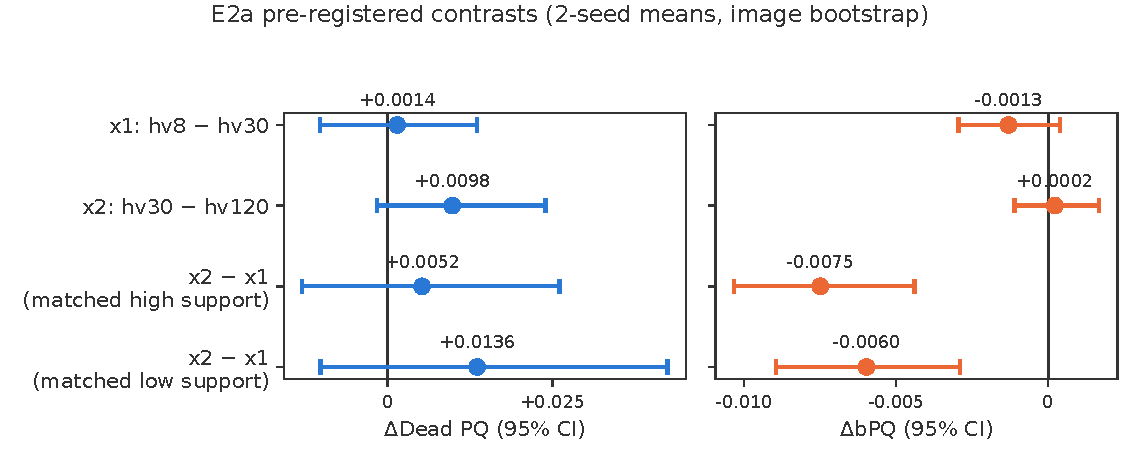
\includegraphics[width=\linewidth]{figs/e2a_contrasts_en.pdf}
\caption{Dead PQ and bPQ deltas with image-bootstrap intervals for the four contrasts. All four Dead intervals cross zero; both scale contrasts have bPQ intervals entirely below zero.}
\label{fig:e2a}
\end{figure}

Four separable findings emerge\cite{hvres}. (1)~Lowering the threshold at x1 is not a substitute for scale: the Dead delta flips sign across seeds ($-0.00138$ / $+0.00426$) and bPQ drops in both. (2)~Within x2 the threshold shows a candidate signal: hv30 yields higher official Dead PQ than hv120 in both seeds (mean $+0.00982$), but the interval crosses zero and strict Dead PQ is inconsistent across seeds. (3)~At matched native support the scale contrasts retain the bPQ penalty --- both bPQ intervals lie entirely below zero with both seeds negative --- while official Dead stays positive on average and \textbf{strict Dead is negative in all four seed pairs}; official and strict endpoints must be reported together. (4)~These contrasts support no causal claim: matching the threshold removes one confound, but scale still changes sampling, features and target discretisation, and the training schedule (learning rate $5.16\times10^{-6}$ at encoder unfreezing) is untested.

Object-level statistics qualify the threshold effect. With the fixed 741 interior Dead instances as denominator, the matched rate rises from 61.27\% to 70.99\% when the working scale increases at matched support; within x2, lowering the threshold moves the mean interior matched count from 526.0 to 526.5 (one extra object across both seeds). The $+0.00982$ official Dead gain is therefore not explained by recovering many more interior objects; the remaining difference most likely lies in mask shape and false-positive structure, which are not decomposed here. Border Dead matching likewise follows scale (40.21\%$\to$48.25\%) and is barely affected by the threshold.

\subsection{Decisions and the gate-A arithmetic}

E2a leads to three standing decisions: the default \code{hv\_min\_size=30} is unchanged; x2\_hv30 is retained as a frozen mechanism reference; and no number from this round is published as a three-split result. For the DSB line, pre-registered gate A evaluates a frozen rule at the E2a point estimates: the x1 threshold move reproduces $r/R = 0.00144/0.01503 = 9.59\%$ of the x2 Dead gain --- below both the 50\% switching threshold and the 90\% full-explanation demotion threshold, with a bPQ penalty of $-0.00130$. The DSB base remains x1\_hv30, and the architecture line is not demoted. The ratio is an evaluation of the frozen rule at the observed estimates, not a causal estimate of the threshold's contribution.

\section{DSB: four pre-registered gates for the Dead-specialist branch}

\subsection{Design and gate logic}

DSB's hypothesis chain: \emph{if} Dead and common classes compete for shared-decoder capacity at the gradient level (H1), \emph{then} an in-model Dead expert branch --- an NP+HV two-channel head supervised only on Dead-positive images, merged into the base instance set as in EF-P2 --- could recover interior Dead recall without hurting aggregate metrics (H2). Design points: the encoder and the existing NP/HV/TP branches remain untouched; there is no over-sampling (balanced sampling was already shown not to help) and no pos-weight (batches that are 97\% pure negative would corrupt the BatchNorm running statistics); loss masking is used instead. A literature check found no direct prior work on class-decoupled experts for nuclei instance segmentation under the official PanNuke protocol; the nearest analogues are classification-domain MoE work\cite{gsmoe,semimoe}. The full design, budget and stop rules were frozen in the pre-registered spec\cite{dsbspec}.

Under spec \S6, four gates must all pass before any GPU training; any failure closes the line with only mechanism evidence retained. The CPU implementation (model, targets, losses, TTA, CLI, merge selection, montage and the four gate scripts) was completed test-first, task by task; the branch was merged into master after the gates closed, as tested tooling --- it has never been trained.

\begin{table}[H]
\centering\small
\caption{The four gates and their pre-frozen continuation conditions (spec \S6, abridged).}
\label{tab:gates}
\begin{tabularx}{\linewidth}{lYY}\toprule
Gate & Checks & Pre-frozen condition\\\midrule
A & E2a threshold arithmetic & $\geq$50\% reproduction switches the base; $\geq$90\% with no performance penalty demotes the architecture line\\
B & Gradient-conflict probe & negative-cosine batch fraction $\geq$30\%, or significantly negative layers\\
C & L0 decision-decoupling ceiling & training-free per-class thresholds reaching $\Delta$Dead $\geq+0.005$ at a bPQ penalty $\leq$0.001 would close the line\\
D & Dead oracle ceiling & $\Delta$Dead $\geq+0.01$ when unmatched interior Dead are inserted at IoU 0.7\\\bottomrule
\end{tabularx}
\end{table}

\subsection{Gates A, C and D}

\textbf{Gate A (proceed; base x1\_hv30).} The arithmetic is as given above; the inputs were re-derived bit-exactly against the frozen E2a snapshot.

\textbf{Gate C (proceed).} Sweeping a Dead-specific decode threshold $\tau_{\mathrm{dead}}\in\{0.5,0.4,0.35,0.3\}$ over validation fold 2 (0.5 = baseline) shows that Dead PQ rises from 0.16386 to at most 0.16601 ($\tau=0.4$), a peak $\Delta$Dead of $+0.00214$ with $\Delta$bPQ $+1.1\times10^{-5}$ --- far below the $+0.005$ closing threshold, so a training-free threshold change does not remove the need for architecture-level decoupling. The baseline Dead PQ matches the official evaluation bit-exactly; the dev-eval menu's re-decode path perturbs the mPQ/bPQ baselines at the $10^{-7}$ level, so only its Dead PQ values are quoted.

\textbf{Gate D (pass).} Inserting all 267 unmatched interior Dead GT instances of fold 2 as oracles shrunk to IoU 0.7 raises Dead PQ from 0.16386 to 0.31992 ($\Delta$Dead $+0.15606$, bPQ $+0.00145$, mPQ $+0.00231$); the exact-mask variant gives $+0.24533$. The ceiling is an order of magnitude above the $+0.01$ threshold: recovering missed interior Dead offers far more headroom than any post-hoc adjustment --- consistent with the diagnosis that Dead is primarily a detection problem.

\subsection{Gate B: the VOID first run and the amended measurement}

Gate B measures the gradient cosine between the Dead-pixel loss group and the common-class loss group at a frozen split-1 checkpoint, using disjoint masks, one forward pass and separate backward passes, with the composite cosine taken over the shared decoder parameters. A conflict is declared if the negative-cosine batch fraction is $\geq$30\% or if any layers are significantly negative.

The first run (00:58) was declared VOID rather than a failure: the pre-frozen plan specified ``the first 256 fold-1 images in order'', which are all Breast tissue and contain exactly one Dead-positive image; 63 of 64 batches therefore contribute structurally zero gradients, which are counted as non-conflicts and cap the conflict fraction at 1/64 before any gradient statistics are measured. The single informative batch shows a decoder-composite cosine of $+0.269$. The probe implementation was verified to be correct; the defect lay in the frozen sampling design and in the accounting of zero-gradient batches. Spec \S10's stop rule was not triggered. The amendment --- Dead-stratified seeded sampling covering all 65 Dead-positive images, denominators over Dead-active batches with $n_{\mathrm{active}}<16$ void, plus the per-layer one-sided $t$ clause with Holm correction --- was registered in the ledger with four new tests before the rerun; the rerun was approved and required only a few minutes of GPU time.

\begin{table}[H]
\centering\small
\caption{Gate B amended rerun: all 65 Dead-positive images covered, 64/64 batches Dead-active, batch size 4. Decoder composite aggregates the skip, NP, HV and TP shared parameters.}
\label{tab:gateb}
\begin{tabular}{lrrr}\toprule
Parameter group & mean per-batch cosine & negative batches & conflict fraction\\\midrule
encoder & $+0.406$ & 0/64 & 0.000\\
skip adapters & $+0.608$ & 0/64 & 0.000\\
NP branch & $+0.917$ & 0/64 & 0.000\\
HV branch & $+0.760$ & 0/64 & 0.000\\
TP branch & $+0.196$ & 7/64 & 0.109\\
decoder composite & $+0.749$ & 0/64 & 0.000\\\bottomrule
\end{tabular}
\end{table}

\begin{figure}[H]
\centering
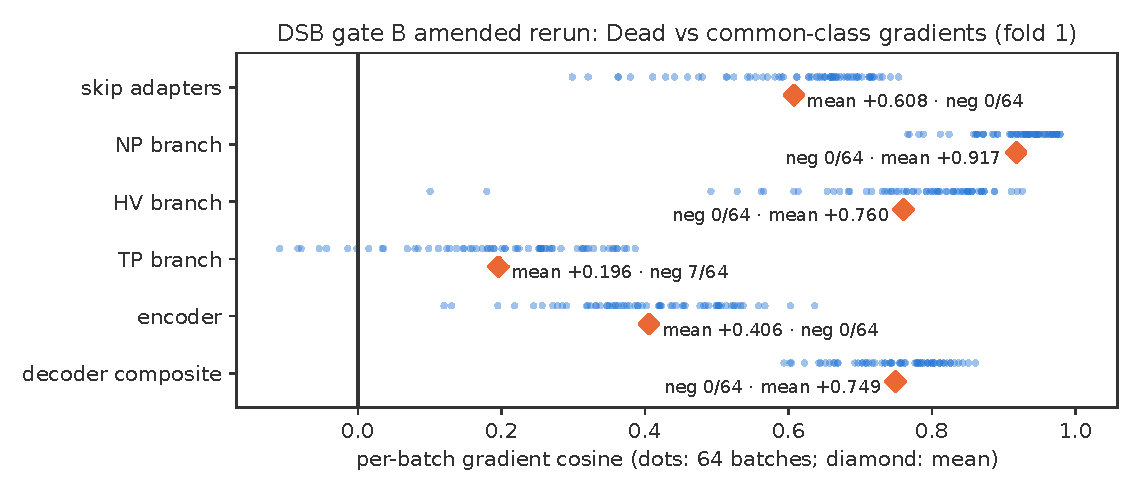
\includegraphics[width=\linewidth]{figs/gate_b_cosines_en.pdf}
\caption{Per-batch gradient cosines in the amended gate-B rerun. Dots: 64 Dead-positive batches; diamonds: means. Every dot lies right of zero; only the TP branch has negative batches (7).}
\label{fig:gateb}
\end{figure}

The amended rerun gives a decisive result: the decoder-composite cosine has mean $+0.749$, per-batch min $+0.594$, median $+0.760$ and max $+0.861$, with \textbf{0 of 64 batches negative} (conflict fraction 0 against the 0.30 threshold; if the true rate were $\geq$30\%, the probability of observing 0/64 is about $10^{-10}$). All six module means are positive, every per-layer one-sided $t$ is positive (decoder composite $t=+89.6$), and no group is significantly negative under Holm. The single informative batch of the first run ($+0.269$) is therefore not an artefact, and Gate B fails the pre-registered conflict criterion.

The measurement covers the converged checkpoint trained with the same recipe (with a sibling-seed checkpoint as fallback); early-training dynamics and loss magnitudes lie outside its scope. The directional conclusion is that, at the trained optimum, improving Dead pixels pushes the shared weights in roughly the same direction as improving common-class pixels. H1 is therefore unsupported, and the premise for specialist decoupling is absent.

\subsection{Closure under the pre-registered stop rule}

Spec \S10 pre-registered that any gate failure closes the line without proceeding to GPU training. After gate B failed, the smoke, dev and confirmatory rounds were all cancelled, and the prepared dev-round queue script remained unused. The four gates nevertheless leave a consistent mechanistic picture: the Dead deficit is a detection-recall problem --- pixel re-weighting and balanced sampling were already falsified, decision-threshold decoupling yields at most $+0.002$, the gradient-conflict premise for architectural decoupling fails, and the detection-level oracle ceiling is $+0.156$. None of these four directions supplies the remedy; that requires either new detection supervision or data (route C), or accepting a two-stage candidate merge together with its measured cost (route B).

\section{E0: the inference cost of the two-model system}

Whereas E2a and the DSB gates inform the decision whether to train, E0 informs the decision whether to deploy. The protocol is fixed: one shared A100-SXM4-80GB, batch 32, 16 decode workers, and wall-clock timing of the unmodified \code{predict\_fold} in 256-image chunks over the 2,523 images of fold 2 (the training fold of the timed split2\_seed1 pair; the cost is checkpoint-independent, no test fold is read, and no endpoint is evaluated). The CPU fusion replays the frozen split2\_seed19 EF-P2 deployment call per image and reproduces its 1,542 additions exactly; the timed path is the deployment path.

\begin{table}[H]
\centering\small
\caption{E0 per-arm timings; best rep by throughput per arm; ratios over x1; fusion is single-threaded CPU.}
\label{tab:e0}
\begin{tabular}{lrrrr}\toprule
Stage & ms/img & img/s & peak GiB & vs x1\\\midrule
x1 & 15.50 & 64.4 & 4.76 & 1.00\\
x2-du2 (GPU) & 52.88 & 18.9 & 12.91 & 3.41\\
x1-TTA (GPU) & 72.33 & 13.8 & 4.93 & 4.67\\
fusion (CPU) & 25.97 & --- & --- & 1.68\\
two-model total & 94.35 & --- & --- & \textbf{6.09}\\\bottomrule
\end{tabular}
\end{table}

\begin{figure}[H]
\centering
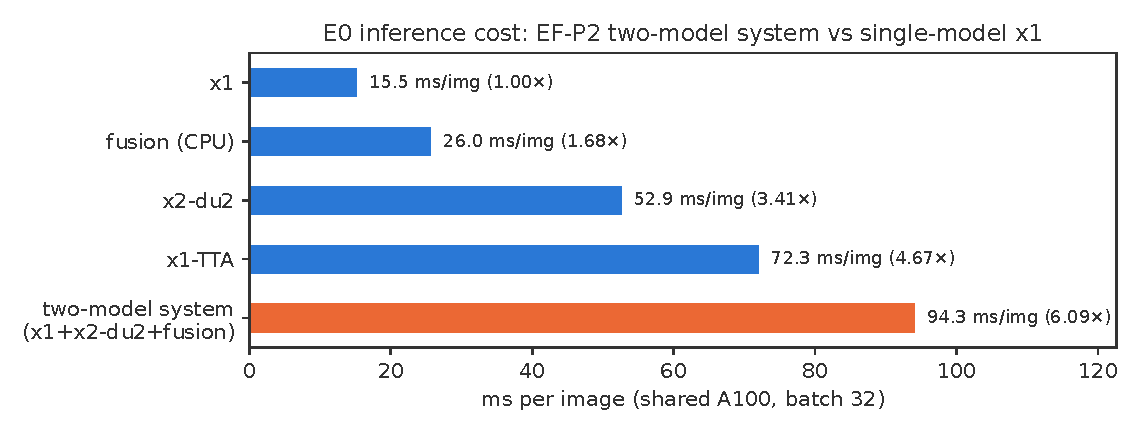
\includegraphics[width=\linewidth]{figs/e0_cost_en.pdf}
\caption{Per-image wall time per stage and the ratio to single-model x1. The two-model system sums x1, x2-du2 and CPU fusion.}
\label{fig:e0}
\end{figure}

The two-model system totals 94.35\,ms/img, \textbf{6.09$\times$} single-model x1; for reference, x1's own TTA costs 4.67$\times$. Absolute milliseconds vary with co-tenant load on the shared GPU (x1 means 10.7--15.5 across four launch windows at load 19--46), but the \emph{ratios} are stable across windows (x2/x1 3.1--3.4; two-model/x1 6.1--6.3; TTA most sensitive at 3.3--4.7). Two protocol notes. First, the frozen artifact's precision label says fp32 although the forward pass actually runs the \code{predict\_fold} bf16-autocast path; all arms share that path, so the ratios are unaffected, and the script label was corrected after the round. Second, the first fusion-timing attempt mistakenly decompressed an npz member separately for every instance (1--27\,s/img); the measurement was repeated after the arrays had been materialised, and the final numbers are bound to the command log.

Under the pre-registered E0 rule --- absent a performance--cost advantage, EF-P2 remains mechanism evidence or a teacher candidate --- EF-P2 is repositioned accordingly: the Dead gain is real, but a deployment claim would carry the $\sim$6$\times$ inference cost, about 1.3$\times$ that of plain x1-TTA, which cannot add Dead detections. The M/S relabelling step was not timed separately (it is a CPU operation of the same order as fusion); model loading, evaluation and multi-process fusion parallelism are excluded, and the exclusions are documented.

\section{Full-repository consistency audit}

On the evening of October 8, three independently run read-only LLM audit agents, together with manual re-derivation, checked the documentation against the code, the documented numbers against the artifacts, and the code against the recorded runs; the full test suite was also run. The central finding is that \textbf{all main results reproduce}: the gate verdicts are bit-consistent with the ledger, the 6.09$\times$ figure re-derives from cost.json, every stage-report/HV-controls/P0--P3 table is exact, and the protocol rules (official evaluator, last checkpoint, 3-split means, no released-checkpoint test results) hold throughout. The post-audit suite passes \textbf{271 tests}.

Corrections and rebuilds: the CellViT-UNI three-split bPQ mean changes 0.6654$\to$\textbf{0.6653} (mean of rounded values replaced by the exact mean); the recovery negative result is restated as ``per-fold maximum regression $-0.0012$''; the KongNet train-fold F1 margin is $\geq$0.12 (minimum 0.124); the CellViT real-domain drop 0.152$\to$0.154; plus a dozen transcription-level fixes. Two artifacts lost on both machines (the fold-3 failure inventory and split2\_seed2's du2/du2lev test evals) were rebuilt from retained deterministic predictions, reproducing the recorded numbers exactly (du2 0.48682/0.65836/0.15259; lever $+0.00157$/$+0.00238$/$+0.00071$; all nine grid verdicts unchanged), with SHA-256 sidecars binding provenance. As an engineering safeguard, \code{fold\_guard} was added: four dev/probe scripts now refuse to run on the test fold of their own run or on unverifiable split ids, and the dev-eval menus are pinned by input hashes and refuse to overwrite existing outputs. The pillar-A CONCH probe outputs were never cached anywhere and remain the only unverifiable entries, now flagged as such. Every correction was re-derived from artifacts before editing; no experimental verdict changed.

\section{Discussion and next steps}

\subsection{Limitations}

\begin{enumerate}
\item \textbf{E2a is single-split, two-seed.} All contrasts are computed on the split-1 validation fold; bootstrap intervals cover image resampling only, and all four Dead intervals cross zero, so the within-x2 threshold effect remains a candidate signal pending three-split confirmation.
\item \textbf{Gate B covers the converged checkpoint only.} Early-training dynamics and loss magnitudes lie outside its scope; the governing spec was frozen before measurement.
\item \textbf{DSB's H2 was never tested.} The line closed at the pre-training gates; the result rules out the decoupling premise but says nothing about the effectiveness of the expert branch.
\item \textbf{E0 is single-machine wall-clock on a shared GPU.} Absolute ms do not transfer directly; ratios were stable across observed windows; loading, evaluation and parallel fusion are excluded.
\item \textbf{No new three-split test scores.} The results are either validation-fold mechanism findings or corrections and repositioning of existing ones; test-fold reuse caveats carry over from stage report III.
\end{enumerate}

\subsection{Next steps}

Within the review's route map\cite{next}, this stage completed the mechanism-attribution and inference-cost items. Priorities are unchanged: first the E1 blind audit of validation candidates (x1-accepted, x2-only accepted, x2-only rejected, random background; expert adjudication including ``undecidable in this field'') to decompose EF-P2's unmatched additions into debris, shape mismatch and suspected annotation gaps; then, if supported, route B's cross-fit utility learning (a $P(\mathrm{match})\cdot E[\mathrm{IoU}\mid\mathrm{match}]>q/2$ proxy) against frozen EF-P2, low-dimensional regression and same-compute TTA/ensemble controls. Route A's crop-consistency mechanism experiments and route C's cross-modal supervision remain conditional. The retained gate tooling (stratified montage, gradient probe, oracle ceiling) is reusable in all of them.

\section{Conclusion}

This stage produced three concrete answers rather than new test scores. First, the HV support threshold is a real but minor confound: lowering it at x1 reproduces 9.59\% of the x2 Dead gain, and at matched support the scale contrast retains the full bPQ penalty, most of the Dead gain, and negative strict Dead in all four seed pairs --- the bulk of the scale effect lies elsewhere. Second, the Dead-specialist premise is falsified: gradients of the Dead and common-class pixel groups are strongly aligned at the trained optimum (composite cosine $+0.749$, zero negative batches), which, together with the falsified re-weighting, the $+0.002$ ceiling of threshold decoupling and the $+0.156$ detection-level oracle headroom, points to \emph{new detection supervision or data}, rather than reallocated capacity, as the direction required for improving Dead; the line was closed by the pre-registered stop rule without any GPU training time. Third, the two-model system measures 6.09$\times$ single-model inference, confirming EF-P2's position as mechanism evidence and a teacher candidate. The full-repository audit confirms that the main results reproduce and corrects the historical record. Together, the mechanism findings, the measured inference cost and the corrected record form the current baseline of the project.

\appendix
\section{Files, numbers and reproduction}

All table numbers in this report are generated by \code{scripts/report4\_numbers.py} from frozen artifacts; \code{scripts/verify\_report4.py} independently recomputes them from the rawest available layer (eight audit evaluation \code{summary.json} files, the five gate JSONs, \code{cost.json}, and the audit-affected test summaries), cross-checks them to within $10^{-12}$, and emits the portable snapshot \code{verified\_numbers.json} (included here; 96 endpoint cells verified). Bootstrap intervals are carried from the frozen E2a snapshot with recorded SHA-256s, not resampled. Gate-B per-batch cosines and per-layer $t$ statistics recompute exactly from the serialised lists; the gate-A ratio and E0 ratios re-derive from raw numbers. The research log\cite{findings} documents the process but is not a numerical source.

On October 8, 2026, the full regression suite passed 271 tests with 64 warnings (Python 3.10, torch 2.5.1+cu124, numpy 1.23.5; no dependencies installed or upgraded). The figure script follows stage report III's Chinese-font and Type-42 embedding conventions; the numbers plotted in the figures match the CSVs in \code{figs/}.

\begin{table}[H]
\centering\footnotesize
\caption{Main artifacts, relative to the repository root; \code{runs/} is local and not distributed with Git.}
\begin{tabularx}{\linewidth}{lY}\toprule
Path & Role in this report\\\midrule
\code{runs/hv\_threshold\_controls\_20261006/} & E2a's eight training arms: configs, logs, original and audit evaluations.\\
\code{runs/analysis/hv\_threshold\_controls\_20261006/} & E2a frozen numbers snapshot and bootstraps.\\
\code{runs/analysis/dsb\_gates\_20261007/} & Gate JSONs and ledger; \code{gate\_b\_v2.json} is canonical for gate B; the VOID first-run artifacts are retained.\\
\code{runs/analysis/inference\_cost\_20261008/} & E0 timings, commands and attempt log.\\
\code{runs/analysis/report4\_numbers.txt} & Per-table number snapshot for this report.\\\bottomrule
\end{tabularx}
\end{table}

From the repository root, in the pinned environment:
\begin{quote}\small
\texttt{python scripts/report4\_numbers.py}\\
\texttt{python scripts/verify\_report4.py}\\
\texttt{python scripts/make\_report\_figures4.py}\\
\texttt{python -m pytest -q}
\end{quote}
The verification scripts fail immediately with an explicit error on missing artifacts or numeric mismatches, and modify nothing. Re-running historical evaluations requires the matching source snapshot or an explicitly registered re-derivation output; provenance checks must not be disabled.

\begin{thebibliography}{9}
\raggedright
\bibitem{reports} Project bdd26. Stage report III: cross-scale candidate filtering and area filtering[R]. 2026-10-06. \code{docs/report/stage_report_3/}.
\bibitem{next} Project bdd26. Research review and next-stage routes (2026-10-06)[R]. \code{docs/RESEARCH_NEXT_2026-10-06.md}.
\bibitem{hvplan} Project bdd26. HV-threshold four-arm controls: pre-registered plan[R]. 2026-10-06. \code{docs/superpowers/plans/2026-10-06-hv-threshold-controls.md}.
\bibitem{hvres} Project bdd26. HV-threshold controls: results and mechanism analysis[R]. 2026-10-07. \code{docs/HV_CONTROLS_RESULTS_2026-10-07.md}.
\bibitem{dsbspec} Project bdd26. Dead-specialist branch (DSB): design spec and implementation plan[R]. 2026-10-07. \code{docs/superpowers/specs/2026-10-07-dead-specialist-branch-design.md}; \code{docs/superpowers/plans/2026-10-07-dead-specialist-branch.md}.
\bibitem{findings} Project bdd26. Research log: entries of 2026-10-06 to 10-08[R]. \code{docs/findings.md}.
\bibitem{pannuke} GAMPER J, ALEMI KOOHBANANI N, BENES K, et al. PanNuke Dataset Extension, Insights and Baselines[EB/OL]. 2020[2026-10-06]. \url{https://arxiv.org/abs/2003.10778}.
\bibitem{uni} CHEN R J, DING T, LU M Y, et al. Towards a general-purpose foundation model for computational pathology[J]. Nature Medicine, 2024, 30(3): 850--862. DOI: \href{https://doi.org/10.1038/s41591-024-02857-3}{10.1038/s41591-024-02857-3}.
\bibitem{cellvit} H\"ORST F, REMPE M, HEINE L, et al. CellViT: Vision Transformers for precise cell segmentation and classification[J]. Medical Image Analysis, 2024, 94: 103143. DOI: \href{https://doi.org/10.1016/j.media.2024.103143}{10.1016/j.media.2024.103143}.
\bibitem{gsmoe} GS-MoE: generalist--specialist branching recovering low-prevalence classes (project shorthand from the DSB spec)[EB/OL]. arXiv:2609.18688, 2026[2026-10-07]. \url{https://arxiv.org/abs/2609.18688}.
\bibitem{semimoe} Semi-MoE: task-level experts for semi-supervised segmentation (project shorthand from the DSB spec)[EB/OL]. arXiv:2509.13834, 2025[2026-10-07]. \url{https://arxiv.org/abs/2509.13834}.
\end{thebibliography}
\end{document}
